\documentclass[1p]{elsarticle_modified}
%\bibliographystyle{elsarticle-num}

%\usepackage[colorlinks]{hyperref}
%\usepackage{abbrmath_seonhwa} %\Abb, \Ascr, \Acal ,\Abf, \Afrak
\usepackage{amsfonts}
\usepackage{amssymb}
\usepackage{amsmath}
\usepackage{amsthm}
\usepackage{scalefnt}
\usepackage{amsbsy}
\usepackage{kotex}
\usepackage{caption}
\usepackage{subfig}
\usepackage{color}
\usepackage{graphicx}
\usepackage{xcolor} %% white, black, red, green, blue, cyan, magenta, yellow
\usepackage{float}
\usepackage{setspace}
\usepackage{hyperref}

\usepackage{tikz}
\usetikzlibrary{arrows}

\usepackage{multirow}
\usepackage{array} % fixed length table
\usepackage{hhline}

%%%%%%%%%%%%%%%%%%%%%
\makeatletter
\renewcommand*\env@matrix[1][\arraystretch]{%
	\edef\arraystretch{#1}%
	\hskip -\arraycolsep
	\let\@ifnextchar\new@ifnextchar
	\array{*\c@MaxMatrixCols c}}
\makeatother %https://tex.stackexchange.com/questions/14071/how-can-i-increase-the-line-spacing-in-a-matrix
%%%%%%%%%%%%%%%

\usepackage[normalem]{ulem}

\newcommand{\msout}[1]{\ifmmode\text{\sout{\ensuremath{#1}}}\else\sout{#1}\fi}
%SOURCE: \msout is \stkout macro in https://tex.stackexchange.com/questions/20609/strikeout-in-math-mode

\newcommand{\cancel}[1]{
	\ifmmode
	{\color{red}\msout{#1}}
	\else
	{\color{red}\sout{#1}}
	\fi
}

\newcommand{\add}[1]{
	{\color{blue}\uwave{#1}}
}

\newcommand{\replace}[2]{
	\ifmmode
	{\color{red}\msout{#1}}{\color{blue}\uwave{#2}}
	\else
	{\color{red}\sout{#1}}{\color{blue}\uwave{#2}}
	\fi
}

\newcommand{\Sol}{\mathcal{S}} %segment
\newcommand{\D}{D} %diagram
\newcommand{\A}{\mathcal{A}} %arc


%%%%%%%%%%%%%%%%%%%%%%%%%%%%%5 test

\def\sl{\operatorname{\textup{SL}}(2,\Cbb)}
\def\psl{\operatorname{\textup{PSL}}(2,\Cbb)}
\def\quan{\mkern 1mu \triangleright \mkern 1mu}

\theoremstyle{definition}
\newtheorem{thm}{Theorem}[section]
\newtheorem{prop}[thm]{Proposition}
\newtheorem{lem}[thm]{Lemma}
\newtheorem{ques}[thm]{Question}
\newtheorem{cor}[thm]{Corollary}
\newtheorem{defn}[thm]{Definition}
\newtheorem{exam}[thm]{Example}
\newtheorem{rmk}[thm]{Remark}
\newtheorem{alg}[thm]{Algorithm}

\newcommand{\I}{\sqrt{-1}}
\begin{document}

%\begin{frontmatter}
%
%\title{Boundary parabolic representations of knots up to 8 crossings}
%
%%% Group authors per affiliation:
%\author{Yunhi Cho} 
%\address{Department of Mathematics, University of Seoul, Seoul, Korea}
%\ead{yhcho@uos.ac.kr}
%
%
%\author{Seonhwa Kim} %\fnref{s_kim}}
%\address{Center for Geometry and Physics, Institute for Basic Science, Pohang, 37673, Korea}
%\ead{ryeona17@ibs.re.kr}
%
%\author{Hyuk Kim}
%\address{Department of Mathematical Sciences, Seoul National University, Seoul 08826, Korea}
%\ead{hyukkim@snu.ac.kr}
%
%\author{Seokbeom Yoon}
%\address{Department of Mathematical Sciences, Seoul National University, Seoul, 08826,  Korea}
%\ead{sbyoon15@snu.ac.kr}
%
%\begin{abstract}
%We find all boundary parabolic representation of knots up to 8 crossings.
%
%\end{abstract}
%\begin{keyword}
%    \MSC[2010] 57M25 
%\end{keyword}
%
%\end{frontmatter}

%\linenumbers
%\tableofcontents
%
\newcommand\colored[1]{\textcolor{white}{\rule[-0.35ex]{0.8em}{1.4ex}}\kern-0.8em\color{red} #1}%
%\newcommand\colored[1]{\textcolor{white}{ #1}\kern-2.17ex	\textcolor{white}{ #1}\kern-1.81ex	\textcolor{white}{ #1}\kern-2.15ex\color{red}#1	}

{\Large $\underline{11a_{258}~(K11a_{258})}$}

\setlength{\tabcolsep}{10pt}
\renewcommand{\arraystretch}{1.6}
\vspace{1cm}\begin{tabular}{m{100pt}>{\centering\arraybackslash}m{274pt}}
\multirow{5}{120pt}{
	\centering
	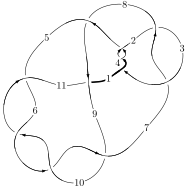
\includegraphics[width=112pt]{../../../GIT/diagram.site/Diagrams/png/507_11a_258.png}\\
\ \ \ A knot diagram\footnotemark}&
\allowdisplaybreaks
\textbf{Linearized knot diagam} \\
\cline{2-2}
 &
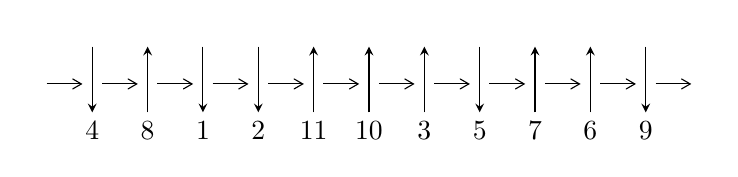
\begin{tikzpicture}[x=20pt, y=17pt]
	% nodes
	\node (C0) at (0, 0) {};
	\node (C1) at (1, 0) {};
	\node (C1U) at (1, +1) {};
	\node (C1D) at (1, -1) {4};

	\node (C2) at (2, 0) {};
	\node (C2U) at (2, +1) {};
	\node (C2D) at (2, -1) {8};

	\node (C3) at (3, 0) {};
	\node (C3U) at (3, +1) {};
	\node (C3D) at (3, -1) {1};

	\node (C4) at (4, 0) {};
	\node (C4U) at (4, +1) {};
	\node (C4D) at (4, -1) {2};

	\node (C5) at (5, 0) {};
	\node (C5U) at (5, +1) {};
	\node (C5D) at (5, -1) {11};

	\node (C6) at (6, 0) {};
	\node (C6U) at (6, +1) {};
	\node (C6D) at (6, -1) {10};

	\node (C7) at (7, 0) {};
	\node (C7U) at (7, +1) {};
	\node (C7D) at (7, -1) {3};

	\node (C8) at (8, 0) {};
	\node (C8U) at (8, +1) {};
	\node (C8D) at (8, -1) {5};

	\node (C9) at (9, 0) {};
	\node (C9U) at (9, +1) {};
	\node (C9D) at (9, -1) {7};

	\node (C10) at (10, 0) {};
	\node (C10U) at (10, +1) {};
	\node (C10D) at (10, -1) {6};

	\node (C11) at (11, 0) {};
	\node (C11U) at (11, +1) {};
	\node (C11D) at (11, -1) {9};
	\node (C12) at (12, 0) {};

	% arrows
	\draw[->,>={angle 60}]
	(C0) edge (C1) (C1) edge (C2) (C2) edge (C3) (C3) edge (C4) (C4) edge (C5) (C5) edge (C6) (C6) edge (C7) (C7) edge (C8) (C8) edge (C9) (C9) edge (C10) (C10) edge (C11) (C11) edge (C12) ;	\draw[->,>=stealth]
	(C1U) edge (C1D) (C2D) edge (C2U) (C3U) edge (C3D) (C4U) edge (C4D) (C5D) edge (C5U) (C6D) edge (C6U) (C7D) edge (C7U) (C8U) edge (C8D) (C9D) edge (C9U) (C10D) edge (C10U) (C11U) edge (C11D) ;
	\end{tikzpicture} \\
\hhline{~~} \\& 
\textbf{Solving Sequence} \\ \cline{2-2} 
 &
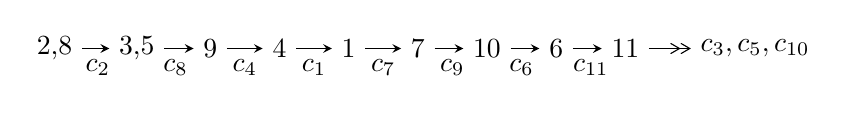
\begin{tikzpicture}[x=25pt, y=7pt]
	% node
	\node (A0) at (-1/8, 0) {2,8};
	\node (A1) at (17/16, 0) {3,5};
	\node (A2) at (17/8, 0) {9};
	\node (A3) at (25/8, 0) {4};
	\node (A4) at (33/8, 0) {1};
	\node (A5) at (41/8, 0) {7};
	\node (A6) at (49/8, 0) {10};
	\node (A7) at (57/8, 0) {6};
	\node (A8) at (65/8, 0) {11};
	\node (C1) at (1/2, -1) {$c_{2}$};
	\node (C2) at (13/8, -1) {$c_{8}$};
	\node (C3) at (21/8, -1) {$c_{4}$};
	\node (C4) at (29/8, -1) {$c_{1}$};
	\node (C5) at (37/8, -1) {$c_{7}$};
	\node (C6) at (45/8, -1) {$c_{9}$};
	\node (C7) at (53/8, -1) {$c_{6}$};
	\node (C8) at (61/8, -1) {$c_{11}$};
	\node (A9) at (10, 0) {$c_{3},c_{5},c_{10}$};

	% edge
	\draw[->,>=stealth]	
	(A0) edge (A1) (A1) edge (A2) (A2) edge (A3) (A3) edge (A4) (A4) edge (A5) (A5) edge (A6) (A6) edge (A7) (A7) edge (A8) ;
	\draw[->>,>={angle 60}]	
	(A8) edge (A9);
\end{tikzpicture} \\ 

\end{tabular} \\

\footnotetext{
The image of knot diagram is generated by the software ``\textbf{Draw programme}" developed by Andrew Bartholomew(\url{http://www.layer8.co.uk/maths/draw/index.htm\#Running-draw}), where we modified some parts for our purpose(\url{https://github.com/CATsTAILs/LinksPainter}).
}\phantom \\ \newline 
\centering \textbf{Ideals for irreducible components\footnotemark of $X_{\text{par}}$} 
 
\begin{align*}
I^u_{1}&=\langle 
4.93541\times10^{32} u^{40}+2.04760\times10^{32} u^{39}+\cdots+1.23008\times10^{33} b-8.08350\times10^{33},\\
\phantom{I^u_{1}}&\phantom{= \langle  }1.21871\times10^{33} u^{40}-1.85520\times10^{33} u^{39}+\cdots+2.46016\times10^{33} a+1.04083\times10^{34},\;u^{41}- u^{40}+\cdots+8 u-16\rangle \\
\\
I^v_{1}&=\langle 
a,\;b-1,\;v^4- v^3+v^2+1\rangle \\
\end{align*}
\raggedright * 2 irreducible components of $\dim_{\mathbb{C}}=0$, with total 45 representations.\\
\footnotetext{All coefficients of polynomials are rational numbers. But the coefficients are sometimes approximated in decimal forms when there is not enough margin.}
\newpage
\renewcommand{\arraystretch}{1}
\centering \section*{I. $I^u_{1}= \langle 4.94\times10^{32} u^{40}+2.05\times10^{32} u^{39}+\cdots+1.23\times10^{33} b-8.08\times10^{33},\;1.22\times10^{33} u^{40}-1.86\times10^{33} u^{39}+\cdots+2.46\times10^{33} a+1.04\times10^{34},\;u^{41}- u^{40}+\cdots+8 u-16 \rangle$}
\flushleft \textbf{(i) Arc colorings}\\
\begin{tabular}{m{7pt} m{180pt} m{7pt} m{180pt} }
\flushright $a_{2}=$&$\begin{pmatrix}1\\0\end{pmatrix}$ \\
\flushright $a_{8}=$&$\begin{pmatrix}0\\u\end{pmatrix}$ \\
\flushright $a_{3}=$&$\begin{pmatrix}1\\- u^2\end{pmatrix}$ \\
\flushright $a_{5}=$&$\begin{pmatrix}-0.495378 u^{40}+0.754100 u^{39}+\cdots+8.36593 u-4.23073\\-0.401227 u^{40}-0.166461 u^{39}+\cdots+3.25878 u+6.57153\end{pmatrix}$ \\
\flushright $a_{9}=$&$\begin{pmatrix}0.00964588 u^{40}+0.868205 u^{39}+\cdots+3.33085 u-12.4271\\-0.279000 u^{40}+0.570378 u^{39}+\cdots+6.14986 u-4.36198\end{pmatrix}$ \\
\flushright $a_{4}=$&$\begin{pmatrix}-0.896605 u^{40}+0.587639 u^{39}+\cdots+11.6247 u+2.34080\\-0.401227 u^{40}-0.166461 u^{39}+\cdots+3.25878 u+6.57153\end{pmatrix}$ \\
\flushright $a_{1}=$&$\begin{pmatrix}-0.896605 u^{40}+0.587639 u^{39}+\cdots+11.6247 u+2.34080\\-0.623981 u^{40}+0.594016 u^{39}+\cdots+8.61517 u-1.62808\end{pmatrix}$ \\
\flushright $a_{7}=$&$\begin{pmatrix}- u\\u^3+u\end{pmatrix}$ \\
\flushright $a_{10}=$&$\begin{pmatrix}0.181324 u^{40}+0.551451 u^{39}+\cdots+0.442667 u-9.89004\\-0.175096 u^{40}+0.493041 u^{39}+\cdots+5.13059 u-4.57783\end{pmatrix}$ \\
\flushright $a_{6}=$&$\begin{pmatrix}-0.295942 u^{40}+0.237376 u^{39}+\cdots+3.40554 u+0.455300\\-0.311321 u^{40}-0.0909921 u^{39}+\cdots+2.02971 u+5.46031\end{pmatrix}$ \\
\flushright $a_{11}=$&$\begin{pmatrix}-0.248888 u^{40}-0.460318 u^{39}+\cdots-0.398174 u+9.13315\\-0.0375077 u^{40}-0.244171 u^{39}+\cdots-1.75912 u+2.99026\end{pmatrix}$\\ \flushright $a_{11}=$&$\begin{pmatrix}-0.248888 u^{40}-0.460318 u^{39}+\cdots-0.398174 u+9.13315\\-0.0375077 u^{40}-0.244171 u^{39}+\cdots-1.75912 u+2.99026\end{pmatrix}$\\&\end{tabular}
\flushleft \textbf{(ii) Obstruction class $= -1$}\\~\\
\flushleft \textbf{(iii) Cusp Shapes $= 0.312617 u^{40}+1.81495 u^{39}+\cdots+9.58739 u-33.8289$}\\~\\
\newpage\renewcommand{\arraystretch}{1}
\flushleft \textbf{(iv) u-Polynomials at the component}\newline \\
\begin{tabular}{m{50pt}|m{274pt}}
Crossings & \hspace{64pt}u-Polynomials at each crossing \\
\hline $$\begin{aligned}c_{1},c_{3},c_{4}\end{aligned}$$&$\begin{aligned}
&u^{41}-5 u^{40}+\cdots-3 u+1
\end{aligned}$\\
\hline $$\begin{aligned}c_{2},c_{7}\end{aligned}$$&$\begin{aligned}
&u^{41}+u^{40}+\cdots+8 u+16
\end{aligned}$\\
\hline $$\begin{aligned}c_{5},c_{6},c_{9}\\c_{10}\end{aligned}$$&$\begin{aligned}
&u^{41}+2 u^{40}+\cdots-3 u-1
\end{aligned}$\\
\hline $$\begin{aligned}c_{8}\end{aligned}$$&$\begin{aligned}
&u^{41}+2 u^{40}+\cdots-20 u-100
\end{aligned}$\\
\hline $$\begin{aligned}c_{11}\end{aligned}$$&$\begin{aligned}
&u^{41}-12 u^{40}+\cdots+549 u-131
\end{aligned}$\\
\hline
\end{tabular}\\~\\
\newpage\renewcommand{\arraystretch}{1}
\flushleft \textbf{(v) Riley Polynomials at the component}\newline \\
\begin{tabular}{m{50pt}|m{274pt}}
Crossings & \hspace{64pt}Riley Polynomials at each crossing \\
\hline $$\begin{aligned}c_{1},c_{3},c_{4}\end{aligned}$$&$\begin{aligned}
&y^{41}-41 y^{40}+\cdots-13 y-1
\end{aligned}$\\
\hline $$\begin{aligned}c_{2},c_{7}\end{aligned}$$&$\begin{aligned}
&y^{41}+27 y^{40}+\cdots-960 y-256
\end{aligned}$\\
\hline $$\begin{aligned}c_{5},c_{6},c_{9}\\c_{10}\end{aligned}$$&$\begin{aligned}
&y^{41}+48 y^{40}+\cdots-7 y-1
\end{aligned}$\\
\hline $$\begin{aligned}c_{8}\end{aligned}$$&$\begin{aligned}
&y^{41}-24 y^{40}+\cdots-163800 y-10000
\end{aligned}$\\
\hline $$\begin{aligned}c_{11}\end{aligned}$$&$\begin{aligned}
&y^{41}-12 y^{40}+\cdots+112237 y-17161
\end{aligned}$\\
\hline
\end{tabular}\\~\\
\newpage\flushleft \textbf{(vi) Complex Volumes and Cusp Shapes}
$$\begin{array}{c|c|c}  
\text{Solutions to }I^u_{1}& \I (\text{vol} + \sqrt{-1}CS) & \text{Cusp shape}\\
 \hline 
\begin{aligned}
u &= \phantom{-}1.04360\phantom{ +0.000000I} \\
a &= -0.918815\phantom{ +0.000000I} \\
b &= \phantom{-}1.34522\phantom{ +0.000000I}\end{aligned}
 & -3.09864\phantom{ +0.000000I} & -0.703580\phantom{ +0.000000I} \\ \hline\begin{aligned}
u &= -0.280650 + 1.032300 I \\
a &= \phantom{-}0.113218 - 0.945326 I \\
b &= \phantom{-}0.451556 + 0.680540 I\end{aligned}
 & -0.98467 - 2.16041 I & \phantom{-}0.30534 + 3.36601 I \\ \hline\begin{aligned}
u &= -0.280650 - 1.032300 I \\
a &= \phantom{-}0.113218 + 0.945326 I \\
b &= \phantom{-}0.451556 - 0.680540 I\end{aligned}
 & -0.98467 + 2.16041 I & \phantom{-}0.30534 - 3.36601 I \\ \hline\begin{aligned}
u &= -0.636469 + 0.676356 I \\
a &= -0.663046 + 0.390386 I \\
b &= \phantom{-}1.123470 - 0.320823 I\end{aligned}
 & -8.62893 + 1.18234 I & -6.12242 + 0.09680 I \\ \hline\begin{aligned}
u &= -0.636469 - 0.676356 I \\
a &= -0.663046 - 0.390386 I \\
b &= \phantom{-}1.123470 + 0.320823 I\end{aligned}
 & -8.62893 - 1.18234 I & -6.12242 - 0.09680 I \\ \hline\begin{aligned}
u &= \phantom{-}0.067485 + 1.087720 I \\
a &= -1.345840 - 0.268602 I \\
b &= -1.365970 + 0.031939 I\end{aligned}
 & -3.50700 + 1.95785 I & -4.15911 - 3.79195 I \\ \hline\begin{aligned}
u &= \phantom{-}0.067485 - 1.087720 I \\
a &= -1.345840 + 0.268602 I \\
b &= -1.365970 - 0.031939 I\end{aligned}
 & -3.50700 - 1.95785 I & -4.15911 + 3.79195 I \\ \hline\begin{aligned}
u &= \phantom{-}0.053492 + 1.097010 I \\
a &= -0.119204 + 0.861224 I \\
b &= \phantom{-}0.644526 - 0.652721 I\end{aligned}
 & -3.46087 - 0.57126 I & -6.38744 + 1.36032 I \\ \hline\begin{aligned}
u &= \phantom{-}0.053492 - 1.097010 I \\
a &= -0.119204 - 0.861224 I \\
b &= \phantom{-}0.644526 + 0.652721 I\end{aligned}
 & -3.46087 + 0.57126 I & -6.38744 - 1.36032 I \\ \hline\begin{aligned}
u &= -0.231068 + 1.076220 I \\
a &= -1.18409 + 0.88552 I \\
b &= -1.359660 - 0.109695 I\end{aligned}
 & -9.84300 - 4.44580 I & -7.49047 + 4.00982 I\\
 \hline 
 \end{array}$$\newpage$$\begin{array}{c|c|c}  
\text{Solutions to }I^u_{1}& \I (\text{vol} + \sqrt{-1}CS) & \text{Cusp shape}\\
 \hline 
\begin{aligned}
u &= -0.231068 - 1.076220 I \\
a &= -1.18409 - 0.88552 I \\
b &= -1.359660 + 0.109695 I\end{aligned}
 & -9.84300 + 4.44580 I & -7.49047 - 4.00982 I \\ \hline\begin{aligned}
u &= \phantom{-}0.575963 + 0.681143 I \\
a &= \phantom{-}0.654397 + 0.985833 I \\
b &= \phantom{-}0.064994 - 0.588385 I\end{aligned}
 & -5.44874 + 2.20051 I & -0.49288 - 3.58387 I \\ \hline\begin{aligned}
u &= \phantom{-}0.575963 - 0.681143 I \\
a &= \phantom{-}0.654397 - 0.985833 I \\
b &= \phantom{-}0.064994 + 0.588385 I\end{aligned}
 & -5.44874 - 2.20051 I & -0.49288 + 3.58387 I \\ \hline\begin{aligned}
u &= -1.179440 + 0.158362 I \\
a &= -0.994717 + 0.088396 I \\
b &= \phantom{-}1.409360 - 0.075417 I\end{aligned}
 & -5.20973 + 3.10308 I & -5.68137 - 4.55677 I \\ \hline\begin{aligned}
u &= -1.179440 - 0.158362 I \\
a &= -0.994717 - 0.088396 I \\
b &= \phantom{-}1.409360 + 0.075417 I\end{aligned}
 & -5.20973 - 3.10308 I & -5.68137 + 4.55677 I \\ \hline\begin{aligned}
u &= \phantom{-}0.353950 + 1.159500 I \\
a &= \phantom{-}0.079020 + 1.089230 I \\
b &= \phantom{-}0.450262 - 0.797995 I\end{aligned}
 & -2.77750 + 5.51756 I & -3.79773 - 7.77564 I \\ \hline\begin{aligned}
u &= \phantom{-}0.353950 - 1.159500 I \\
a &= \phantom{-}0.079020 - 1.089230 I \\
b &= \phantom{-}0.450262 + 0.797995 I\end{aligned}
 & -2.77750 - 5.51756 I & -3.79773 + 7.77564 I \\ \hline\begin{aligned}
u &= \phantom{-}0.005676 + 1.227250 I \\
a &= -0.228021 - 0.942171 I \\
b &= \phantom{-}0.720117 + 0.732589 I\end{aligned}
 & -11.55890 + 2.26622 I & -7.69126 - 0.18572 I \\ \hline\begin{aligned}
u &= \phantom{-}0.005676 - 1.227250 I \\
a &= -0.228021 + 0.942171 I \\
b &= \phantom{-}0.720117 - 0.732589 I\end{aligned}
 & -11.55890 - 2.26622 I & -7.69126 + 0.18572 I \\ \hline\begin{aligned}
u &= -0.383325 + 1.244490 I \\
a &= \phantom{-}0.043543 - 1.163710 I \\
b &= \phantom{-}0.463101 + 0.864387 I\end{aligned}
 & -10.75100 - 7.67961 I & -5.88345 + 5.74816 I\\
 \hline 
 \end{array}$$\newpage$$\begin{array}{c|c|c}  
\text{Solutions to }I^u_{1}& \I (\text{vol} + \sqrt{-1}CS) & \text{Cusp shape}\\
 \hline 
\begin{aligned}
u &= -0.383325 - 1.244490 I \\
a &= \phantom{-}0.043543 + 1.163710 I \\
b &= \phantom{-}0.463101 - 0.864387 I\end{aligned}
 & -10.75100 + 7.67961 I & -5.88345 - 5.74816 I \\ \hline\begin{aligned}
u &= \phantom{-}1.287610 + 0.202232 I \\
a &= -1.055360 - 0.112449 I \\
b &= \phantom{-}1.46107 + 0.09654 I\end{aligned}
 & -13.2971 - 5.0740 I & -7.49177 + 2.86395 I \\ \hline\begin{aligned}
u &= \phantom{-}1.287610 - 0.202232 I \\
a &= -1.055360 + 0.112449 I \\
b &= \phantom{-}1.46107 - 0.09654 I\end{aligned}
 & -13.2971 + 5.0740 I & -7.49177 - 2.86395 I \\ \hline\begin{aligned}
u &= -0.637500 + 0.135734 I \\
a &= \phantom{-}1.71237 - 0.80495 I \\
b &= -0.363345 + 0.258087 I\end{aligned}
 & -7.29387 + 3.70140 I & \phantom{-}0.13489 - 3.24211 I \\ \hline\begin{aligned}
u &= -0.637500 - 0.135734 I \\
a &= \phantom{-}1.71237 + 0.80495 I \\
b &= -0.363345 - 0.258087 I\end{aligned}
 & -7.29387 - 3.70140 I & \phantom{-}0.13489 + 3.24211 I \\ \hline\begin{aligned}
u &= -0.442927 + 0.446451 I \\
a &= \phantom{-}0.885936 - 0.663779 I \\
b &= \phantom{-}0.002285 + 0.351914 I\end{aligned}
 & \phantom{-}0.739118 - 0.963294 I & \phantom{-}5.38374 + 5.24951 I \\ \hline\begin{aligned}
u &= -0.442927 - 0.446451 I \\
a &= \phantom{-}0.885936 + 0.663779 I \\
b &= \phantom{-}0.002285 - 0.351914 I\end{aligned}
 & \phantom{-}0.739118 + 0.963294 I & \phantom{-}5.38374 - 5.24951 I \\ \hline\begin{aligned}
u &= \phantom{-}0.545126 + 0.215241 I \\
a &= \phantom{-}1.37573 + 0.63189 I \\
b &= -0.218730 - 0.254700 I\end{aligned}
 & \phantom{-}0.06188 - 1.89506 I & \phantom{-}3.00107 + 4.96508 I \\ \hline\begin{aligned}
u &= \phantom{-}0.545126 - 0.215241 I \\
a &= \phantom{-}1.37573 - 0.63189 I \\
b &= -0.218730 + 0.254700 I\end{aligned}
 & \phantom{-}0.06188 + 1.89506 I & \phantom{-}3.00107 - 4.96508 I \\ \hline\begin{aligned}
u &= \phantom{-}0.332351 + 0.473594 I \\
a &= -0.483789 - 0.209918 I \\
b &= \phantom{-}0.984199 + 0.167639 I\end{aligned}
 & -1.84031 - 0.69258 I & -6.89864 - 1.74884 I\\
 \hline 
 \end{array}$$\newpage$$\begin{array}{c|c|c}  
\text{Solutions to }I^u_{1}& \I (\text{vol} + \sqrt{-1}CS) & \text{Cusp shape}\\
 \hline 
\begin{aligned}
u &= \phantom{-}0.332351 - 0.473594 I \\
a &= -0.483789 + 0.209918 I \\
b &= \phantom{-}0.984199 - 0.167639 I\end{aligned}
 & -1.84031 + 0.69258 I & -6.89864 + 1.74884 I \\ \hline\begin{aligned}
u &= \phantom{-}0.52227 + 1.35643 I \\
a &= -0.110639 - 1.064090 I \\
b &= -1.49556 + 0.25090 I\end{aligned}
 & -7.31234 + 5.60210 I & \phantom{-0.000000 } 0 \\ \hline\begin{aligned}
u &= \phantom{-}0.52227 - 1.35643 I \\
a &= -0.110639 + 1.064090 I \\
b &= -1.49556 - 0.25090 I\end{aligned}
 & -7.31234 - 5.60210 I & \phantom{-0.000000 } 0 \\ \hline\begin{aligned}
u &= -0.41034 + 1.42300 I \\
a &= -0.140257 + 0.816586 I \\
b &= -1.52685 - 0.19609 I\end{aligned}
 & -10.55130 - 2.41180 I & \phantom{-0.000000 } 0 \\ \hline\begin{aligned}
u &= -0.41034 - 1.42300 I \\
a &= -0.140257 - 0.816586 I \\
b &= -1.52685 + 0.19609 I\end{aligned}
 & -10.55130 + 2.41180 I & \phantom{-0.000000 } 0 \\ \hline\begin{aligned}
u &= -0.60199 + 1.38207 I \\
a &= \phantom{-}0.024627 + 1.133790 I \\
b &= -1.50901 - 0.28951 I\end{aligned}
 & -9.13999 - 9.48739 I & \phantom{-0.000000 } 0 \\ \hline\begin{aligned}
u &= -0.60199 - 1.38207 I \\
a &= \phantom{-}0.024627 - 1.133790 I \\
b &= -1.50901 + 0.28951 I\end{aligned}
 & -9.13999 + 9.48739 I & \phantom{-0.000000 } 0 \\ \hline\begin{aligned}
u &= \phantom{-}0.65669 + 1.41457 I \\
a &= \phantom{-}0.127888 - 1.155240 I \\
b &= -1.52575 + 0.31574 I\end{aligned}
 & -17.2037 + 11.9877 I & \phantom{-0.000000 } 0 \\ \hline\begin{aligned}
u &= \phantom{-}0.65669 - 1.41457 I \\
a &= \phantom{-}0.127888 + 1.155240 I \\
b &= -1.52575 - 0.31574 I\end{aligned}
 & -17.2037 - 11.9877 I & \phantom{-0.000000 } 0 \\ \hline\begin{aligned}
u &= \phantom{-}0.38128 + 1.53983 I \\
a &= \phantom{-}0.017651 - 0.667778 I \\
b &= -1.58265 + 0.18117 I\end{aligned}
 & -19.3092 + 0.9583 I & \phantom{-0.000000 } 0\\
 \hline 
 \end{array}$$\newpage$$\begin{array}{c|c|c}  
\text{Solutions to }I^u_{1}& \I (\text{vol} + \sqrt{-1}CS) & \text{Cusp shape}\\
 \hline 
\begin{aligned}
u &= \phantom{-}0.38128 - 1.53983 I \\
a &= \phantom{-}0.017651 + 0.667778 I \\
b &= -1.58265 - 0.18117 I\end{aligned}
 & -19.3092 - 0.9583 I & \phantom{-0.000000 } 0\\
 \hline 
 \end{array}$$\newpage\newpage\renewcommand{\arraystretch}{1}
\centering \section*{II. $I^v_{1}= \langle a,\;b-1,\;v^4- v^3+v^2+1 \rangle$}
\flushleft \textbf{(i) Arc colorings}\\
\begin{tabular}{m{7pt} m{180pt} m{7pt} m{180pt} }
\flushright $a_{2}=$&$\begin{pmatrix}1\\0\end{pmatrix}$ \\
\flushright $a_{8}=$&$\begin{pmatrix}v\\0\end{pmatrix}$ \\
\flushright $a_{3}=$&$\begin{pmatrix}1\\0\end{pmatrix}$ \\
\flushright $a_{5}=$&$\begin{pmatrix}0\\1\end{pmatrix}$ \\
\flushright $a_{9}=$&$\begin{pmatrix}v\\v\end{pmatrix}$ \\
\flushright $a_{4}=$&$\begin{pmatrix}1\\1\end{pmatrix}$ \\
\flushright $a_{1}=$&$\begin{pmatrix}0\\-1\end{pmatrix}$ \\
\flushright $a_{7}=$&$\begin{pmatrix}v\\0\end{pmatrix}$ \\
\flushright $a_{10}=$&$\begin{pmatrix}v^3+v\\v\end{pmatrix}$ \\
\flushright $a_{6}=$&$\begin{pmatrix}v^3- v^2-1\\v^3\end{pmatrix}$ \\
\flushright $a_{11}=$&$\begin{pmatrix}- v^2\\- v^2-1\end{pmatrix}$\\ \flushright $a_{11}=$&$\begin{pmatrix}- v^2\\- v^2-1\end{pmatrix}$\\&\end{tabular}
\flushleft \textbf{(ii) Obstruction class $= 1$}\\~\\
\flushleft \textbf{(iii) Cusp Shapes $= 4 v^2-5 v-1$}\\~\\
\newpage\renewcommand{\arraystretch}{1}
\flushleft \textbf{(iv) u-Polynomials at the component}\newline \\
\begin{tabular}{m{50pt}|m{274pt}}
Crossings & \hspace{64pt}u-Polynomials at each crossing \\
\hline $$\begin{aligned}c_{1}\end{aligned}$$&$\begin{aligned}
&(u-1)^4
\end{aligned}$\\
\hline $$\begin{aligned}c_{2},c_{7}\end{aligned}$$&$\begin{aligned}
&u^4
\end{aligned}$\\
\hline $$\begin{aligned}c_{3},c_{4}\end{aligned}$$&$\begin{aligned}
&(u+1)^4
\end{aligned}$\\
\hline $$\begin{aligned}c_{5},c_{6}\end{aligned}$$&$\begin{aligned}
&u^4+u^3+3 u^2+2 u+1
\end{aligned}$\\
\hline $$\begin{aligned}c_{8},c_{11}\end{aligned}$$&$\begin{aligned}
&u^4- u^3+u^2+1
\end{aligned}$\\
\hline $$\begin{aligned}c_{9},c_{10}\end{aligned}$$&$\begin{aligned}
&u^4- u^3+3 u^2-2 u+1
\end{aligned}$\\
\hline
\end{tabular}\\~\\
\newpage\renewcommand{\arraystretch}{1}
\flushleft \textbf{(v) Riley Polynomials at the component}\newline \\
\begin{tabular}{m{50pt}|m{274pt}}
Crossings & \hspace{64pt}Riley Polynomials at each crossing \\
\hline $$\begin{aligned}c_{1},c_{3},c_{4}\end{aligned}$$&$\begin{aligned}
&(y-1)^4
\end{aligned}$\\
\hline $$\begin{aligned}c_{2},c_{7}\end{aligned}$$&$\begin{aligned}
&y^4
\end{aligned}$\\
\hline $$\begin{aligned}c_{5},c_{6},c_{9}\\c_{10}\end{aligned}$$&$\begin{aligned}
&y^4+5 y^3+7 y^2+2 y+1
\end{aligned}$\\
\hline $$\begin{aligned}c_{8},c_{11}\end{aligned}$$&$\begin{aligned}
&y^4+y^3+3 y^2+2 y+1
\end{aligned}$\\
\hline
\end{tabular}\\~\\
\newpage\flushleft \textbf{(vi) Complex Volumes and Cusp Shapes}
$$\begin{array}{c|c|c}  
\text{Solutions to }I^v_{1}& \I (\text{vol} + \sqrt{-1}CS) & \text{Cusp shape}\\
 \hline 
\begin{aligned}
v &= -0.351808 + 0.720342 I \\
a &= \phantom{-0.000000 } 0 \\
b &= \phantom{-}1.00000\phantom{ +0.000000I}\end{aligned}
 & -1.43393 + 1.41510 I & -0.82145 - 5.62908 I \\ \hline\begin{aligned}
v &= -0.351808 - 0.720342 I \\
a &= \phantom{-0.000000 } 0 \\
b &= \phantom{-}1.00000\phantom{ +0.000000I}\end{aligned}
 & -1.43393 - 1.41510 I & -0.82145 + 5.62908 I \\ \hline\begin{aligned}
v &= \phantom{-}0.851808 + 0.911292 I \\
a &= \phantom{-0.000000 } 0 \\
b &= \phantom{-}1.00000\phantom{ +0.000000I}\end{aligned}
 & -8.43568 - 3.16396 I & -5.67855 + 1.65351 I \\ \hline\begin{aligned}
v &= \phantom{-}0.851808 - 0.911292 I \\
a &= \phantom{-0.000000 } 0 \\
b &= \phantom{-}1.00000\phantom{ +0.000000I}\end{aligned}
 & -8.43568 + 3.16396 I & -5.67855 - 1.65351 I\\
 \hline 
 \end{array}$$\newpage
\newpage\renewcommand{\arraystretch}{1}
\centering \section*{ III. u-Polynomials}
\begin{tabular}{m{50pt}|m{274pt}}
Crossings & \hspace{64pt}u-Polynomials at each crossing \\
\hline $$\begin{aligned}c_{1}\end{aligned}$$&$\begin{aligned}
&((u-1)^4)(u^{41}-5 u^{40}+\cdots-3 u+1)
\end{aligned}$\\
\hline $$\begin{aligned}c_{2},c_{7}\end{aligned}$$&$\begin{aligned}
&u^4(u^{41}+u^{40}+\cdots+8 u+16)
\end{aligned}$\\
\hline $$\begin{aligned}c_{3},c_{4}\end{aligned}$$&$\begin{aligned}
&((u+1)^4)(u^{41}-5 u^{40}+\cdots-3 u+1)
\end{aligned}$\\
\hline $$\begin{aligned}c_{5},c_{6}\end{aligned}$$&$\begin{aligned}
&(u^4+u^3+3 u^2+2 u+1)(u^{41}+2 u^{40}+\cdots-3 u-1)
\end{aligned}$\\
\hline $$\begin{aligned}c_{8}\end{aligned}$$&$\begin{aligned}
&(u^4- u^3+u^2+1)(u^{41}+2 u^{40}+\cdots-20 u-100)
\end{aligned}$\\
\hline $$\begin{aligned}c_{9},c_{10}\end{aligned}$$&$\begin{aligned}
&(u^4- u^3+3 u^2-2 u+1)(u^{41}+2 u^{40}+\cdots-3 u-1)
\end{aligned}$\\
\hline $$\begin{aligned}c_{11}\end{aligned}$$&$\begin{aligned}
&(u^4- u^3+u^2+1)(u^{41}-12 u^{40}+\cdots+549 u-131)
\end{aligned}$\\
\hline
\end{tabular}\newpage\renewcommand{\arraystretch}{1}
\centering \section*{ IV. Riley Polynomials}
\begin{tabular}{m{50pt}|m{274pt}}
Crossings & \hspace{64pt}Riley Polynomials at each crossing \\
\hline $$\begin{aligned}c_{1},c_{3},c_{4}\end{aligned}$$&$\begin{aligned}
&((y-1)^4)(y^{41}-41 y^{40}+\cdots-13 y-1)
\end{aligned}$\\
\hline $$\begin{aligned}c_{2},c_{7}\end{aligned}$$&$\begin{aligned}
&y^4(y^{41}+27 y^{40}+\cdots-960 y-256)
\end{aligned}$\\
\hline $$\begin{aligned}c_{5},c_{6},c_{9}\\c_{10}\end{aligned}$$&$\begin{aligned}
&(y^4+5 y^3+7 y^2+2 y+1)(y^{41}+48 y^{40}+\cdots-7 y-1)
\end{aligned}$\\
\hline $$\begin{aligned}c_{8}\end{aligned}$$&$\begin{aligned}
&(y^4+y^3+3 y^2+2 y+1)(y^{41}-24 y^{40}+\cdots-163800 y-10000)
\end{aligned}$\\
\hline $$\begin{aligned}c_{11}\end{aligned}$$&$\begin{aligned}
&(y^4+y^3+3 y^2+2 y+1)(y^{41}-12 y^{40}+\cdots+112237 y-17161)
\end{aligned}$\\
\hline
\end{tabular}
\vskip 2pc
\end{document}